\documentclass[twocolumn,10pt]{article}
\usepackage{url,graphicx,tabularx,array}%,geometry} %,fullpage,amsfonts,amsmath}
\usepackage{amsmath,amsthm,amsfonts,amssymb,amscd,mathabx,ulem}
\usepackage{fullpage}
\usepackage{lastpage}
\usepackage{enumerate}
\usepackage{fancyhdr}
\usepackage{mathrsfs}
\usepackage[margin=1.5cm]{geometry}
\usepackage{listings}
\usepackage{mathabx}
\usepackage{tikz,pgfplots}
\usepackage{enumitem}
\usepackage{graphicx,wrapfig}
\usepackage{color,hyperref,endnotes}

\usetikzlibrary{arrows,shapes}
\usepackage{tikz-qtree}

%\setlength{\parskip}{1ex} %--skip lines between paragraphs
\setlength{\parindent}{0pt} %--don't indent paragraphs
\setlist{nolistsep}
%-- Commands for header

\definecolor{mygreen}{rgb}{0,0.6,0}
\definecolor{mygray}{rgb}{0.5,0.5,0.5}
\definecolor{mymauve}{rgb}{0.58,0,0.82}
\definecolor{lightgray}{rgb}{.9,.9,.9}
\definecolor{darkgray}{rgb}{.4,.4,.4}
\definecolor{purple}{rgb}{0.65, 0.12, 0.82}

% \renewcommand{\title}[1]{\textbf{#1}\\}
\newcommand{\red}[1]{\textcolor{red}{#1}}
\newcommand{\gray}[1]{\textcolor{gray}{#1}}

\lstset{basicstyle=\footnotesize\ttfamily, 
	tabsize=2,
	language=Python,
	backgroundcolor=\color{lightgray},
	commentstyle=\color{mygreen},
	keywordstyle=\color{blue},
	stringstyle=\color{red}\ttfamily,
	showstringspaces=false,
	breaklines=true
}

\title{CS246: Twitter Purification}
\author{Wen Shi, Zijun Xue, Jennifer Zhang}
\date{June 2014}
\begin{document}
\maketitle

\section*{Abstract}
\section*{Introduction}
\subsection*{Motivation}
\subsection*{Overview}
\section*{Implementation}
\subsection*{Dataset}
\paragraph{} Approximately 800,000 tweets consisting of about 120,000 distinct words were harvested Twitter's sample API\footnote{\href{https://dev.twitter.com/docs/api/1.1/get/statuses/sample}{GET statuses/sample}}. Word tokens were defined as any whitespace delimited string that begins with an alphabet letter and otherwise may include alphanumeric characters, apostrophes, or hyphens. We excluded some Twitter specific tokens, including usernames (strings that begin with @), hashtags (strings that begin with \#), emoticons, and internet urls (\textit{http(s)://...}). All strings were converted to lowercase for analysis. Final corrected output replaced any usernames with \textit{[username]}, and a hardcoded list of laughter tokens were converted to \textit{[laughter]}.\footnote{lmao, lmfao, lolz, lol, rofl, lls, haha}
\subsection*{Dictionary}
\paragraph{} In a standard spellchecker, a word would be searched against an existing dictionary, and skipped over if it exists and corrected if it doesn't. This is, unfortunately, not an acceptable method of attack for correcting tweets. The major issue with this approach is that it assumes a perfect dictionary; given the amount of slang, proper nouns, etc. in tweets, this is not only exceptionally difficult, but constitutes a moving target as new slang and names are propagated daily.
\paragraph{} In the case where a given word already exists in the dictionary, it could easily be a word misuse; aside from common grammatical mistakes such as confounding \textit{your} or \textit{you're}, it is common to intentionally misspell \textit{then} as \textit{den}. Since \textit{den} is a legitimate word in the English language, a normal spellchecker would fail to attempt to correct it. 
\paragraph{} In the case where a word is encountered that does not exist in a dictionary, it is often more appropriate to not apply a correction. Slang and proper nouns abound in Twitter; while the line between a legitimate word versus a misspelling can be blurry, e.g. \textit{want to} vs \textit{wanna}, but a great deal of slang have no `correct' equivalent in a dictionary, e.g. Twitter specific words such as \textit{retweet} as well as many more vulgar examples.
\paragraph{}Nonetheless, a high quality dictionary was desirable for this project. Word candidates that exist in the dictionary can therefore be weighted more heavily, and correctly spelled obscure words can avoid being overwhelmed by exceptionally common words that are closely phonetically related or via edit distance (e.g. \textit{goat} being overwhelmed by the frequency of \textit{got}. Initially, a union of UNIX's dictionary, Google Translate's list of most frequently used words\footnote{\href{https://github.com/first20hours/google-10000-english}{google-10000-english}}, and the most common words from TV and movie scripts\footnote{\href{http://en.wiktionary.org/wiki/Wiktionary:Frequency_lists\#TV_and_movie_scripts}{Wiktionary Frequency Lists}} was used. However, this failed to produce an acceptable dictionary, partially due to the overinclusion of slang and underinclusion of conjugated verbs or plurals. Inevitably, we settled upon using Ispell's english dictionary, which consisted of 143,006 words.\footnote{\href{http://fmg-www.cs.ucla.edu/geoff/ispell-dictionaries.html}{Dictionaries for International Ispell}}
\paragraph{} In the context of Twitter purification, if the given word exists in the dictionary, it is guaranteed a position in the final list of correction candidates, with the same weight as that of the frontrunner candidate (if different). Furthermore, any candidates that exist in the dictionary are weighted more heavily by $+20\%$.
\subsection*{Single word correction}
\subsubsection*{Abbreviations: single word}
\paragraph{} The most common occurrences in the Twitter dataset were crosschecked against the dictionary, and mismatches were examined. Words that are abbreviations for single words\footnote{Common abbreviations for phrases were stored separately for substitution later} such that their distance was judged to be too far for an automated system to determine were listed into a separate reference file\footnote{see Appendix A-1}. This included instances where an abbreviation potentially had multiple interpretations (e.g. \textit{ur} $\rightarrow$ \textit{[your, you're]}).
\paragraph{} When the purifier begins analysis of a word, it is crosschecked against this manually maintained list and makes replacements in the correction candidate list as indicated.
\subsubsection*{Squeeze}
TODO: Zijun
\subsubsection*{Edit distance}
TODO: Zijun
\subsubsection*{Phonetic candidates: Soundex}
TODO: Shi Wen
\subsubsection*{Phonetic candidates: Metaphone}
TODO: Shi Wen
\subsubsection*{Letter similarity: Viterbi}
\paragraph{} Several hundred correction candidates may be found for a word, based on searching within a particular edit distance or the same Soundex/Metaphone class. To trim this list, we first make some intuitive assumptions about the manner in which Twitter users typically misspell their words.
\begin{itemize}
\item Abbreviation: Twitter words are usually shorter than their correct counterparts
\item Letter similarity: the same important letters are usually present in the Twitter word as the correct counterpart. There are a few phonetic exceptions to this, e.g. substituting \textit{d} for \textit{th}, as in \textit{dere} vs \textit{there}.
\item Transposition of remaining significant letters is rare, which makes sense if other letters have already been omitted for brevity.
\end{itemize}
With these observations in mind, we set out to find a reasonable scoring algorithm to measure the similarity between a Twitter word versus its correction candidate.

\paragraph{} The Viterbi algorithm is a dynamic programming algorithm typically used in hidden Markov models, such that it finds the optimal path of hidden states given a set of observations. In implementation, an $n\times m$ matrix $V$ is created, such that $n$ is the number of observations and $m$ is the number of hidden states. Each entry of the matrix is a product of the probability of transitioning from the prior state into that state multiplied by the Viterbi score of the prior state; the maximum of these possibilities is populated into the matrix. Mathematically, where $t$ is the timestep, $i$ is the hidden state, and $j$ is the prior hidden state:
$$V_{ti} = \max\limits_j p(X_t = s_i | X_{t-1} = s_j) V_{t-1,j}$$
When the exact path of hidden states needs to be returned, another matrix with identical dimensions is needed to keep track of which prior state was chosen for each entry.
\paragraph{}In the context of Twitter purification, the Viterbi matrix is constructed such that $n$ is length of the observed tweeted word, and $m$ is the length of the correction candidate. The transition probability to a specific entry is interpreted as the score to match two letters, or to skip a letter in either direction. In the interest of computational simplicity, addition is used as the logarithmic equivalent to multiplication; this is common practice when probability values are involved for better computational handling of small numbers. Thus, where $w$ is the Twitter word and $c$ is the correction candidate:
$$V_{j,i} = \max\begin{cases}
\text{match score between $(w_i,c_j)$} + V_{j-1, i-1}\\
\text{gap penalty of skipping over $w_i$} + V_{j, i-1}\\
\text{gap penalty of skipping over $c_j$} + V_{j-1, i}
\end{cases}$$
The value of $V_{m,n}$ is interpreted as the best match score between $w$ and $c$.
\paragraph{} Transition costs are set in a $27 \times 27$ matrix that indicate the positive score of a match or negative penalty (see Appendix A-2). Since we only have interest in relative scores rather than actual probabilistic values, the individual numbers do not need to be normalized in any sense. The horizontal and vertical gap penalties are $(-1, -0.1)$ respectively, to reflect the fact that Twitter words are more likely to be abbreviated. Both the scoring matrix and appropriate gap penalties were roughly approximated based on observations about misspellings that were encountered, and have a great deal of room for improvement in a more analytic manner.
\paragraph{} An example of calculating the letter similarity of \textit{den} versus correction candidate \textit{then}, excluding irrelevant entries:
$$\begin{array} {c|cccc}
& & d & e & n \\ \hline
& 0 &\leftarrow -1 & \leftarrow -2 &  \leftarrow -3\\
t & \uparrow -0.1 & \nwarrow 4 & & \\
h & \uparrow -0.2 & \uparrow 3.9 & & \\
e & \uparrow -0.3& & \nwarrow 8.9 & \\
n & \uparrow -0.4 & & & \nwarrow 13.9 \\
\end{array}$$
The final similarity score is $13.9 / 15.0$, where 15.0 is the similarity of (\textit{den, den}). Each correction candidate is weighted by their similarity scoring, and any with a similarity score less than 0.7 are thrown out. 
\paragraph{} This algorithm does not behave as well in cases where the Twitter word is longer than the original. In general, this is rare, but a common exception is replacing the IPA phoneme $\alpha$\footnote{\href{http://en.wiktionary.org/wiki/\%C9\%91}{Wiktionary: $\alpha$}} with \textit{aw}, e.g. writing \textit{dawg} instead of \textit{dog}. An idealized version of this algorithm might use phonemes instead of specific letters, but this would require an additional conversion step from a given English word to potential pronunciations. While some phonetic dictionaries for the English language exist\footnote{\href{http://www.speech.cs.cmu.edu/cgi-bin/cmudict}{The CMU Pronouncing Dictionary}}, there would need to be an algorithm that interprets the pronunciation of the obscure, misspellings, or slang among the Twitter input.
\subsubsection*{Word frequency scaling}
\paragraph{}Using Bayes' rule, where $w$ is the tweeted word and $c$ is the candidate correction:
$$\Pr(c|w) \varpropto \Pr(c) \Pr(w|c)$$
$\Pr(w|c)$ represents the weights associated with candidates thus far -- it includes some accounting for edit distance and/or phonetic distance as well as letter similarity to the original. $\Pr(c)$ is now applied using the word frequency of $c$ in the Twitter dataset. A hash table of all words and their respective frequencies was created ahead of time so lookups were $O(1)$. \paragraph{} Originally, the weight was multiplied by the raw word frequency, but this quickly proved to produce undesirable results; it became impossible to prevent common words from overwhelming less common words, e.g. \textit{got} has a word frequency of 13807, and \textit{goat} has a word frequency of 87, approximately 2 orders of magnitudes apart. This particular example isn't troublesome since \textit{goat} exists in the dictionary and would be restored to the candidate list, but this problem is particularly serious for any words that the dictionary does not cover. Therefore, the weight was multiplied by $\ln (\text{word frequency})$ to reduce its impact.
\paragraph{}As a final step, the list of correction candidates are trimmed down to the most promising ones. Suppose that $s_i$ is the highest score out of the correction candidates. Any correction candidates with a score $s_j > 70\% \times s_i$ are kept.
\subsection*{Bigram correction}
TODO: add some subsections here?
\subsubsection*{Substitutions}
\paragraph{} During the analysis for common abbreviations described above, any common abbreviations that map to phrases were stored in a separate reference file. Note that unlike single word abbreviations, these are unambiguous and only map to a single possibility (see Appendix A-3). After single word and bigram correction, laughter tokens and any such abbreviations are substituted with these expansions.
\section*{Discussion and Evaluation}
\subsection*{Single word results}
\paragraph{} 368 of the most frequent Twitter words that did not appear in the dictionary were manually mapped to their correct counterparts. In some cases, there were multiple possible corrections; let us refer to this set of corrections as $L_1$. The single word correction algorithm as detailed above was applied to each word in turn, and the resultant list of candidates $L_2$ was compared with $L_1$. If $L_1\cap L_2 = \emptyset$, then it is counted as an error. The Twitter purification algorithm above produced 76/368 errors.
TODO: Zijun or Shiwen to add some data about comparison with existing spell checker
\subsection*{Bigram results}
\section*{Future work}
TODO: listing any more aspects where it didn't work well
\subsubsection*{Unconventional word tokenization}
\subsubsection*{Obscure vocabulary or slang}
\subsubsection*{Proper nouns and acronyms}
\subsubsection*{Abbreviations}
\subsubsection*{Dictionary}
\section*{Appendix}
\subsection*{A-1 Abbreviations: single word}
\begin{verbatim}
2	to
2	two
2	too
fav	favorite
xd	XD
tl	timeline
ig	instagram
fb	facebook
u	you
r	are
c	see
y	why
ur	your
ur	you're
w	with
bf	boyfriend
gf	girlfriend
bfs	boyfriends
gfs	girlfriends
gr8	great
bc	because
mfs	motherfuckers
mf	motherfucker
rt	retweet
hw	hw
hw	homework
rp	roleplay
da	the
da	da
\end{verbatim}
\subsection*{A-2 Letter match scores}
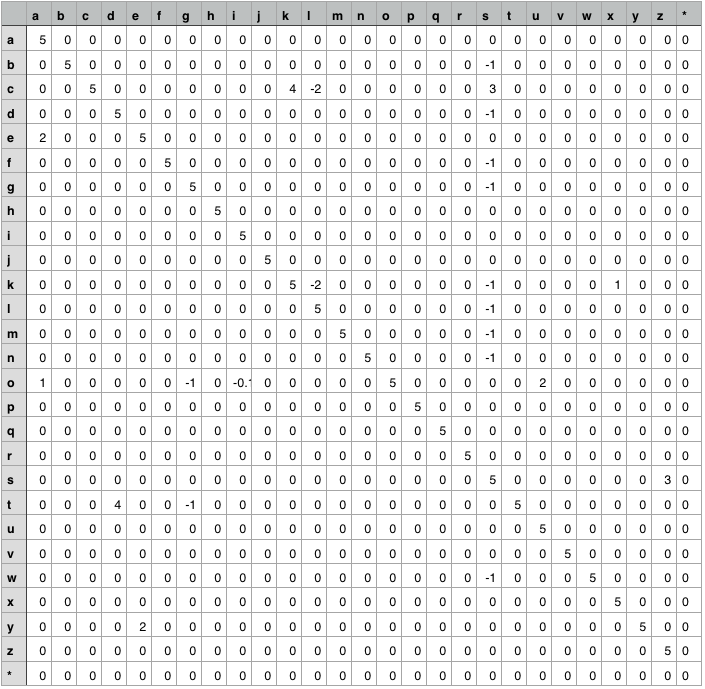
\includegraphics[width=0.5\textwidth]{viterbi_matrix.png}
\subsection*{A-3 Abbreviations: phrases}
\begin{verbatim}
omg	oh my god
idk	I don't know
idek	I don't even know
omfg	oh my fucking god
wtf	what the fuck
smh	shaking my head
ily	I love you
ilysm	I love you so much
tbh	to be honest
idc	I don't care
stfu	shut the fuck up
btw	by the way
ik	I know
idgaf	I don't give a fuck
jk	just kidding
hmu	hit me up
bff	best friend
nvm	never mind
ffs	for fucks sake
oomf	one of my friends
\end{verbatim}
\end{document}